\chapter{Testy urządzenia}
\section{Analiza poboru prądu układu}
Zarówno w trakcie tworzenia pracy jak i jej planowania, zakładano minimalizację zużycia energii przez układ. Dzięki zastosowaniu odpowiednich komponentów, założenie to, zostało spełnione w bardzo dobrym stopniu. W trybie analizy, gdzie urządzenie spędzało znakomitą większość czasu, wartość pobieranego prądu spadała do nawet 200$\mu$A. Dzięki temu, stosując małe ogniwo Li-Pol o pojemności 600mAh, urządzenie mogło czuwać przez nawet 3000 godzin, co daje 125 pełne doby. Najwięcej prądu, pobierało pierwsze wyzwoleie alarmu. Średni jego pobór, sięgał tutaj nawet 50mA, w zależności od czasu potrzebnego na określenie lokalizacji. Kolejne transmisje nie były już tak energochłonne, ponieważ uruchamiany był tylko modem LTE.
\newline
Rysunek \ref{img:current_summary} przedstawia kompletną analizę poboru prądu przez układ. Obszar pierwszy, to obszar inicjalizacji urządzenia. To tutaj ustawiany jest każdy z komponentów i dokonywana jest pierwsza rejestracja do sieci. Należy zauważyć, że w tym miejsciu nie był uruchamiany GPS, co przyspieszyło inicjalizację układu. Strefa ta, jest tzw. selftestem, gwarantującym, że urządzenie będzie działać poprawnie w przypadku wypadku. W strefie drugiej, wszystkie podzespoły, znajdowały się w trybie głębokiego uśpienia. Wbudowane w akcelerometr maszyny stanów, cały czas monitorowały dane w trybie niskiego poboru energii. Na granicy obszarów 2 i 3, nastąpiło przerwanie. Uruchomiło ono procedurę alarmu, wyzwalając buzzer oraz uruchamiając GPS. Obszar 3 stanowiła próba określenia swojego położenia, a następnie przygotowanie i wysłanie wiadomości, poprzedzone rejestracją do sieci komórkowej. W obszarze czwartym, modem przeszedł w tryb uśpienia, a uruchomiony został licznik, który po minucie wyzwoliłby kolejne wysłanie wiadomości. Na granicy stref 4 i 5, nastąpiło przytrzymanie przycisku, które zakończyło alarm i wyłącza buzzer. Układ ponownie przeszedł w tryb analizy danych.
	

\begin{figure}[h]
    \centering
    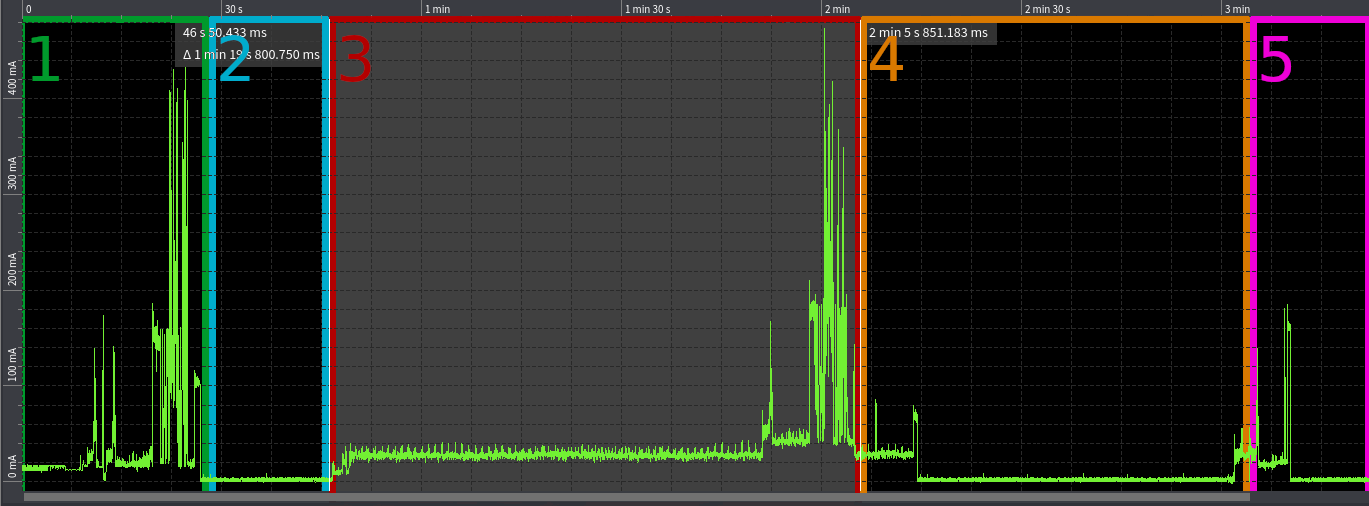
\includegraphics[width=14cm]{Graphics/connection_with_fix_divided.png}
    \caption{Analiza poboru prądu przy użyciu urządzenia otii}
    \label{img:current_summary}
\end{figure}

\section{Testy algorytmów}
Ze względów bezpieczeństwa, maszyny stanów przetestowane zostały poprzez potrząsanie układem w sposób, mający wyzwolić kolejne maszyny. Pierwsza z nich, testująca przekroczenie wartości, wyzwalała się poprawnie. Należy zauważyć, że maszyna testuje sygnał nieprzefiltrowany, porównany na rysunku \ref{img:signal_comparsion}. Wykres niebieski, przedstawia zaszumiony sygnał. Widać jednak na nim, że w momencie wypadku, pojedyncze próbki sięgają wartości $\pm$7g. Po filtracji, wykres czerwony jest znacznie bardziej czytelny, jednak nie występują w nim tak duże wartości przyspieszenia.
\newline
Kolejna z maszyn stanów, wykrywająca przewrócenie roweru, zadziałała w każdym z przypadków. Na rysunku \ref{img:fsm3_recognize} zaznaczono krótki fragment, prowadzący do wyzwolenia maszyny stanów. Ponieważ rower po wypadku, przewrócony był na jeden bok, wartość przyspieszenia w osi Y osiągnęła stałą wartość bliską -1g. Po dwóch minutach w niezminionej pozycji, rower uznany został za przewrócony, co skutkowało przerwaniem i alarmem.
\newline
Ostatnia maszyna stanów, odpowiedzialna za wykrycie uderzenia  i przewrotu również działała poprawnie. Na rysunku \ref{img:fsm4_recognize} kolejne punkty zaznaczają momenty przejścia przez etapy maszyny stanów. Dla czytelności, na przebiegu przedstawiono sygnał przefiltrowany, jednak maszyna stanów, pracując na surowych danych, wykrywa wartości znacznie większe od przefiltrowanych. W jej przypadku, kluczowa jest zmiana znaku przyspieszenia, w stosunkowo niedużym czasie.


\begin{figure}[h]
    \centering
    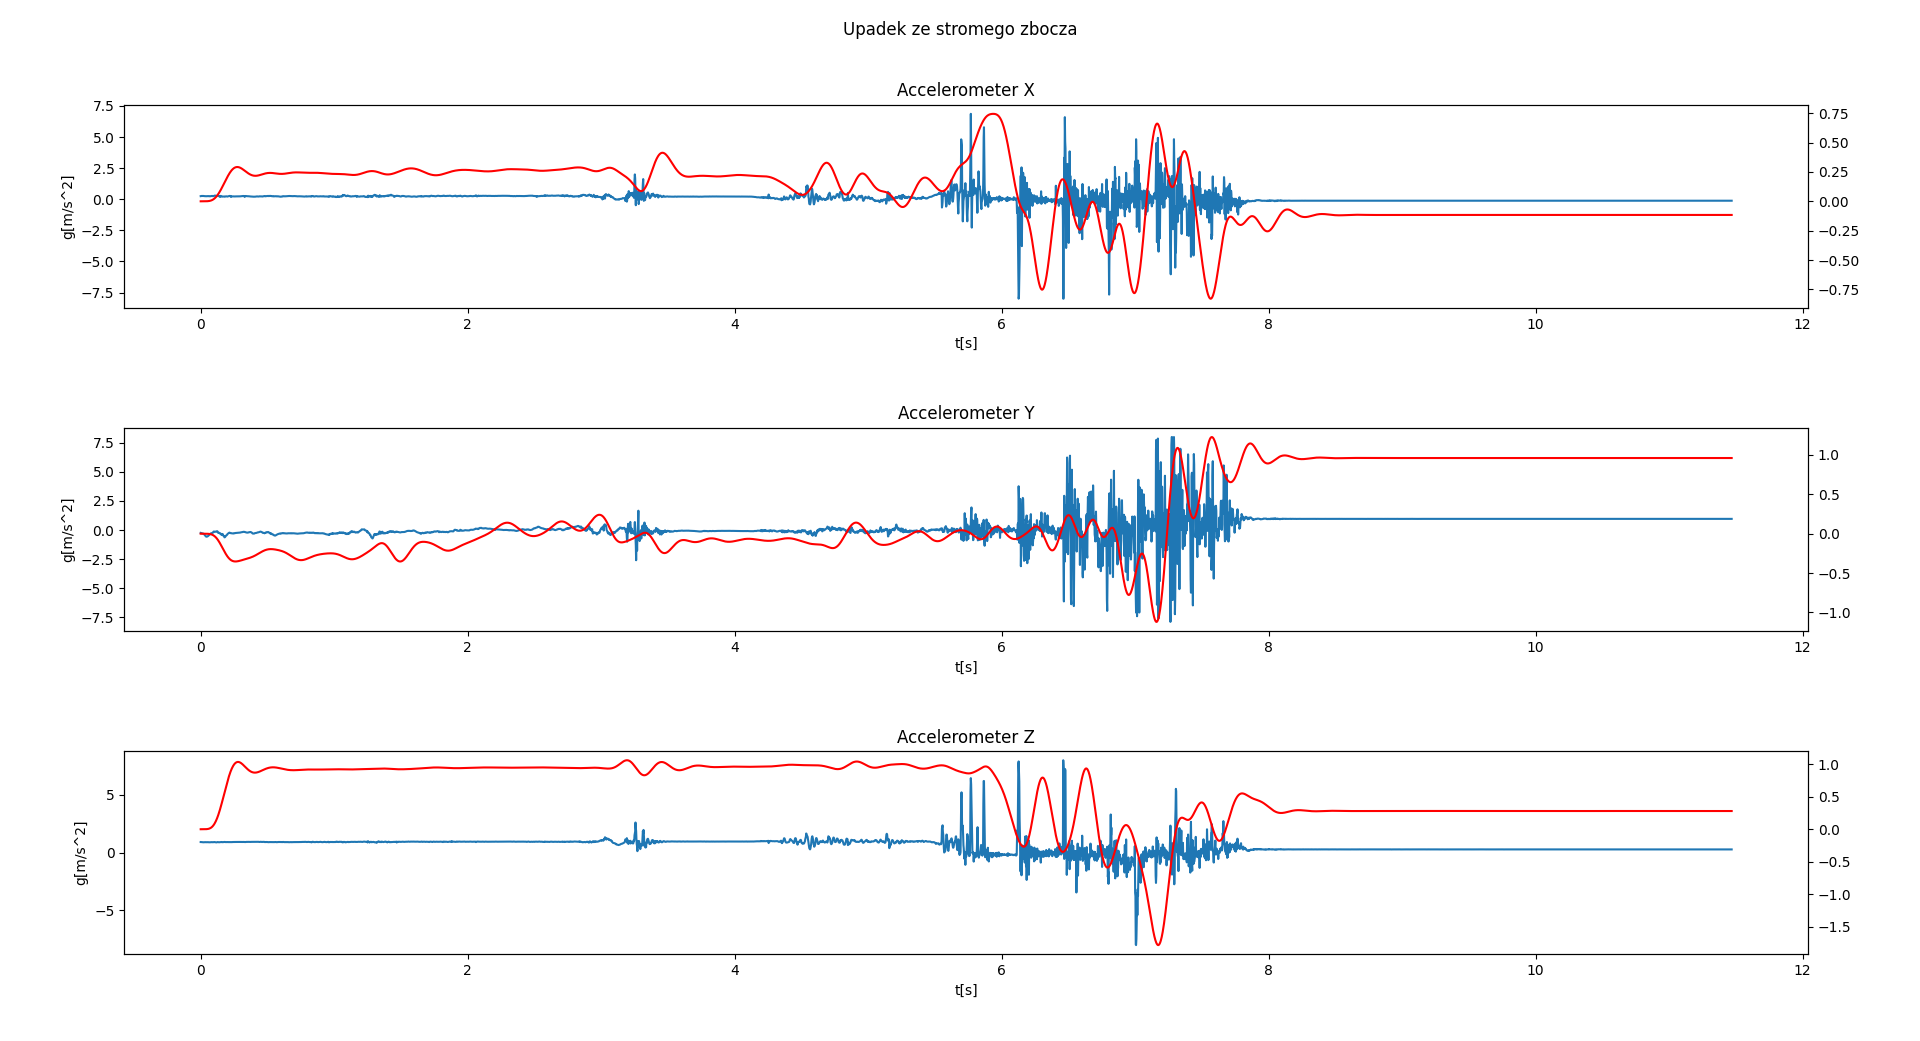
\includegraphics[width=15cm]{Graphics/Before_and_after_filter.png}
    \caption{Porównanie sygnału surowego do sygnału po filtracji}
    \label{img:signal_comparsion}
\end{figure}

\begin{figure}[h]
    \centering
    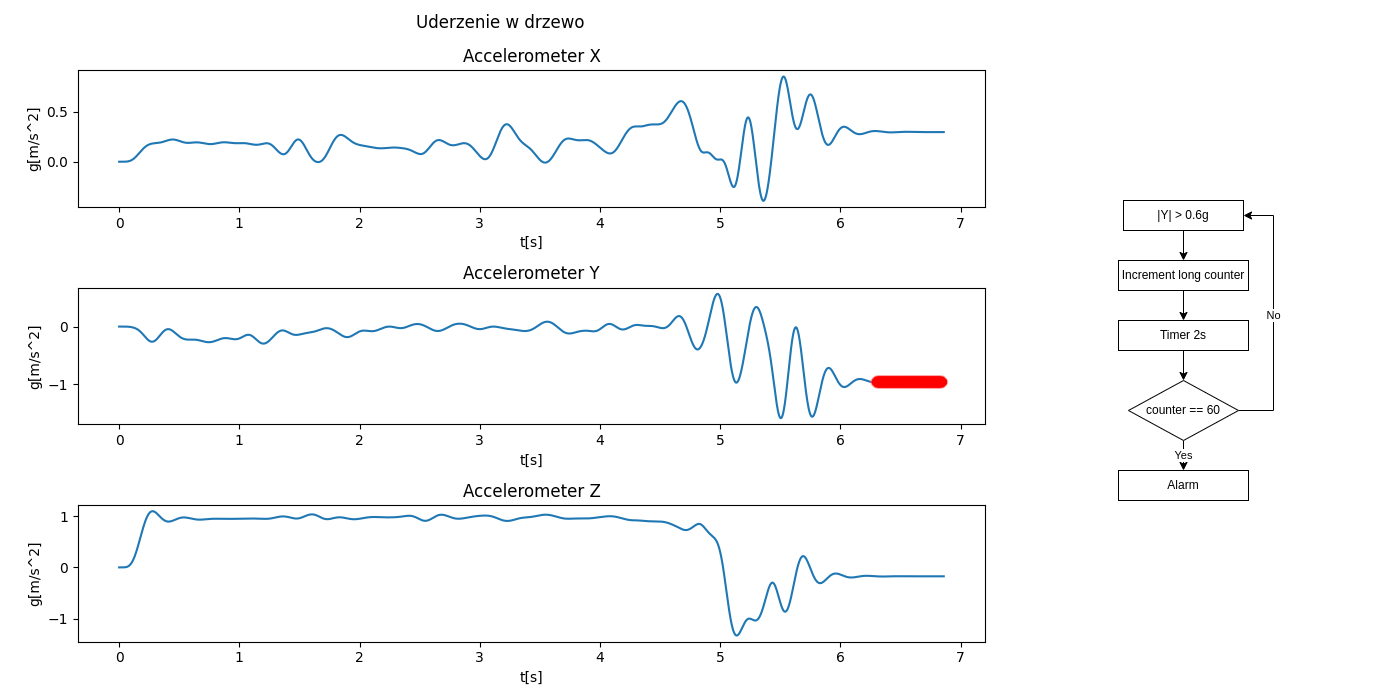
\includegraphics[width=15cm]{Graphics/Tree_title_to_fsm.png}
    \caption{Wyzwolenie maszyny stanów, wykrywającej leżący rower}
    \label{img:fsm3_recognize}
\end{figure}

\begin{figure}[h]
    \centering
    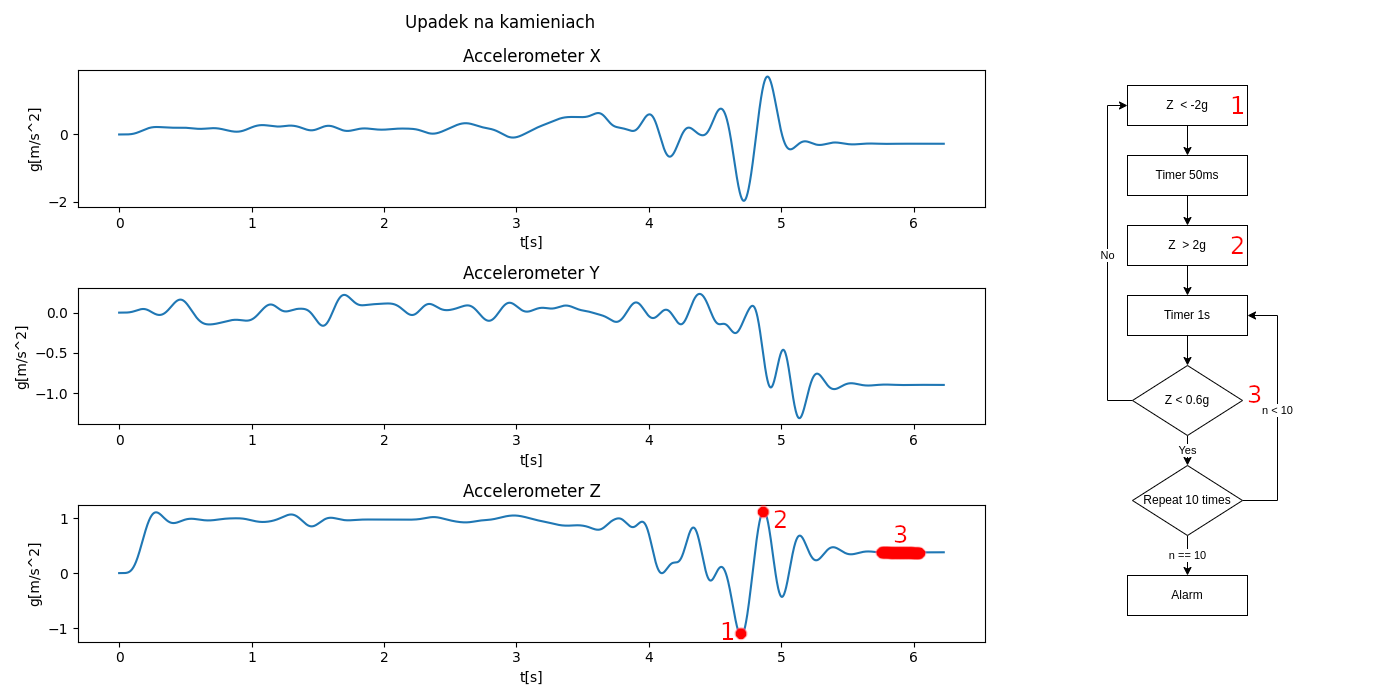
\includegraphics[width=15cm]{Graphics/Stones_title_to_fsm.png}
    \caption{Wyzwolenie maszyny stanów, wykrywająca uderzenie i przewrót}
    \label{img:fsm4_recognize}
\end{figure}